\documentclass[12pt]{article}
\usepackage{times} 			% use Times New Roman font

\usepackage[margin=1in]{geometry}   % sets 1 inch margins on all sides
\usepackage{hyperref}               % for URL formatting
\usepackage[pdftex]{graphicx}       % So includegraphics will work
\setlength{\parskip}{1em}           % skip 1em between paragraphs
\usepackage{indentfirst}            % indent the first line of each paragraph
\usepackage{datetime}
\usepackage[small, bf]{caption}
\usepackage{listings}               % for code listings
\usepackage{xcolor}                 % for styling code
\usepackage{multirow}

%New colors defined below
\definecolor{backcolour}{RGB}{246, 246, 246}   % 0xF6, 0xF6, 0xF6
\definecolor{codegreen}{RGB}{16, 124, 2}       % 0x10, 0x7C, 0x02
\definecolor{codepurple}{RGB}{170, 0, 217}     % 0xAA, 0x00, 0xD9
\definecolor{codered}{RGB}{154, 0, 18}         % 0x9A, 0x00, 0x12

%Code listing style named "gcolabstyle" - matches Google Colab
\lstdefinestyle{gcolabstyle}{
  basicstyle=\ttfamily\small,
  backgroundcolor=\color{backcolour},   
  commentstyle=\itshape\color{codegreen},
  keywordstyle=\color{codepurple},
  stringstyle=\color{codered},
  numberstyle=\ttfamily\footnotesize\color{darkgray}, 
  breakatwhitespace=false,         
  breaklines=true,                 
  captionpos=b,                    
  keepspaces=true,                 
  numbers=left,                    
  numbersep=5pt,                  
  showspaces=false,                
  showstringspaces=false,
  showtabs=false,                  
  tabsize=2
}

\lstset{style=gcolabstyle}      %set gcolabstyle code listing

% to make long URIs break nicely
\makeatletter
\g@addto@macro{\UrlBreaks}{\UrlOrds}
\makeatother

% for fancy page headings
\usepackage{fancyhdr}
\setlength{\headheight}{13.6pt} % to remove fancyhdr warning
\pagestyle{fancy}
\fancyhf{}
\rhead{\small \thepage}
\lhead{\small HW 7\, Venkatesh}  % EDIT THIS, REPLACE # with HW number
\chead{\small CS 532, Fall 2021} 

%-------------------------------------------------------------------------
\begin{document}

% EDIT THE ITEMS HERE
\begin{centering}
{\large\textbf{HW 7\ - Recommendation Systems}}\\ 
Swathi Venkatesh\\
11/29/2021\\
\end{centering}

%-------------------------------------------------------------------------

% The * after \section just says to not number the sections
\section*{Q1}
Find 3 users who are closest to you in terms of age, gender, and occupation.
For each of those 3 users:
\begin{itemize}
        \item \emph{Q. What are their top 3 (favorite) films?}
        \item \emph{Q. What are their bottom 3 (least favorite) films?}
    \end{itemize}
Based on the movie values in those 6 tables (3 users X (favorite + least favorite)), choose a user that you feel is most like you. Feel free to note any outliers (e.g., "I mostly identify with user 123, except I did not like "Ghost" at all"). You can investigate more than just the top 3 and bottom 3 movies to find your best match.

This user is the substitute you.

\subsection*{Answer}

%Python code highlighting
\begin{lstlisting}[language=Python, caption=one.py , label=1st:copy]
#!/usr/local/bin/python3
import pandas as pd

def funcAgeGendOccupation(item,data):

    #load movies data into variables
    movies = {}
    for line in open(str(item)):
        (id, title) = line.split('|')[0:2]
        movies[id] = title
    # Load data
    prefs = {}
    for line in open(str(data)):
        (user, movieid, rating, ts) = line.split('\t')
        prefs.setdefault(user, {})
        prefs[user][movies[movieid]] = float(rating)
    #Load in users
    users = []
    for line in open('movie/u.user'):
        (user, age, gender, occupation, zipcode) = line.split('|')
        dictA = {'user': user, 'age':age, 'gender': gender, 'occupation' :occupation }
        users.append(dictA)
    
    count = 1
    #hold 3 similar user in term of age gender and category
    similarUser =[]
    #Find all users that have things common with me 
    for a in users:
        """
        passed in my age gender and occupation
        to find users of my age gender and occupation category.
        I take only 3 users
        """
        if a['age'] == '23' and a['gender'] == 'F' and a['occupation'] == 'student' and count < 4 :
            similarUser.append(a['user'])
            count += 1
    #print user movie likes
    for a in similarUser:
        """
        Based on similar users like me,
        I obtained these similar users top 3 favorite films 
        """
        if a in prefs:
            #this gets the movie names, and the movie rating per user
            p = pd.DataFrame(list(prefs[a].items()),columns=["Movie Names","Rating"])
            #this sort the users movie list based on rating in decending order
            p.sort_values("Rating",ascending=False, inplace=True)
            #gets the top3 films
            top3 = p.head(3)
            #gets the bottom 3 films
            bottom3 = p.tail(3)
            top3.to_csv("one/"+a+"top3.csv",index=False)
            bottom3.to_csv("one/"+a+"bottom.csv",index=False)
funcAgeGendOccupation('movie/u.item','movie/u.data')


\end{lstlisting}

\begin{table}[ht]
\centering
\caption{Top 3 movies for user 49}
\label{tbl}
\begin{tabular}{|l|l|}
\hline
\textbf{Movie Names} & \textbf{Rating} \\ \hline \hline
Monty Python and the Holy Grail (1974) & 5.0   \\ \hline
Paradise Lost: The Child Murders at Robin Hood Hills (1996) & 5.0   \\ \hline
Clockwork Orange, A (1971) & 5.0  \\ \hline
\end{tabular}
\end{table}

\begin{table}[ht]
\centering
\caption{Bottom 3 movies for user 49}
\label{tb2}
\begin{tabular}{|l|l|}
\hline
\textbf{Movie Names} & \textbf{Rating} \\ \hline \hline
Firm, The (1993) & 1.0   \\ \hline
Long Kiss Goodnight, The (1996) & 1.0   \\ \hline
Terminator 2: Judgment Day (1991) & 1.0  \\ \hline
\end{tabular}
\end{table}

\begin{table}[ht]
\centering
\caption{Top 3 movies for user 159}
\label{tb3}
\begin{tabular}{|l|l|}
\hline
\textbf{Movie Names} & \textbf{Rating} \\ \hline \hline
Grumpier Old Men (1995) & 5.0   \\ \hline
That Old Feeling (1997) & 5.0   \\ \hline
Volcano (1997) & 5.0  \\ \hline
\end{tabular}
\end{table}

\begin{table}[ht]
\centering
\caption{Bottom 3 movies for user 159}
\label{tb4}
\begin{tabular}{|l|l|}
\hline
\textbf{Movie Names} & \textbf{Rating} \\ \hline \hline
Grumpier Old Men (1995) & 1.0   \\ \hline
Soul Food (1997) & 1.0   \\ \hline
Ace Ventura: Pet Detective (1994) & 1.0  \\ \hline
\end{tabular}
\end{table}

\begin{table}[ht]
\centering
\caption{Top 3 movies for user 477}
\label{tb5}
\begin{tabular}{|l|l|}
\hline
\textbf{Movie Names} & \textbf{Rating} \\ \hline \hline
One Fine Day (1996) & 5.0   \\ \hline
Evita (1996) & 5.0   \\ \hline
Grease (1978) & 5.0  \\ \hline
\end{tabular}
\end{table}

\begin{table}[ht]
\centering
\caption{Bottom 3 movies for user 477}
\label{tb6}
\begin{tabular}{|l|l|}
\hline
\textbf{Movie Names} & \textbf{Rating} \\ \hline \hline
Corrina, Corrina (1994) & 4.0   \\ \hline
Black Sheep (1996) & 4.0   \\ \hline
Don Juan DeMarco (1995) & 4.0  \\ \hline
\end{tabular}
\end{table}

\clearpage
\subsection*{Discussion}
\begin{itemize}
        \item \emph{Q. What are their top 3 (favorite) films?}
        \item \emph{Q. What are their bottom 3 (least favorite) films?}
    \end{itemize}
The users top 3 and bottom 3 films are shown in the above tables.

I created a function called funcAgeGendOccupation() ,in line 4. This function takes two parameters of the location of u.item and u.data path. u.user was not going through as a parameter so it is passed directly. 

From lines 6-22  the data from each file is read and stored into dictionary variables. In line 24 -36, I found users that were just as similar to me in age, gender and occupation. I limited this search to find only just 3 similar users to me on line 30. These users where stored in a list variable called similarUser. The line 26 is the variable declaration, while line 35 appends new users to the list in the created variable.

The lines 38 to 53, process the outcomes for top 3 movies and bottom 3 movies for each users found. Using a for loop to retrieve each user, parse this result to ensure that the said user is in prefs dictionary. If present, retrieve the row of the dictionary of that particular user. Using a pandas dataframe in Line 45, parse a list of the row item, so that we can easily sort the data based on values in Rating column in descending order. Retrieve the first three data using pandas .head(3) and the last three data using .tail(3). Save each result as a pandas dataFrame and convert the result to a saved csv file in one/. 

My best substitute user is 159, the movies user hates I hate and the movies the user enjoys I too find them interesting.


\section*{Q2}
Based on the ratings that users have given to the movies, answer the following questions:
\begin{itemize}
        \item \emph{Q: Which 5 users are most correlated to the substitute you (i.e., which 5 users rate movies most similarly to the substitute you?)}
        \item \emph{Q: Which 5 users are least correlated (i.e., negative correlation)?}
    \end{itemize}

\subsection*{Answer}
%Python code highlighting
\begin{lstlisting}[language=Python, caption=two.py , label=2nd:copy]
#!/usr/local/bin/python3
from math import sqrt

def sim_pearson(prefs, p1, p2):
    """
    Returns the Pearson correlation coefficient for p1 and p2.
    """

# Get the list of mutually rated items
    si = {}
    for item in prefs[p1]:
        if item in prefs[p2]:
            si[item] = 1
            
# If they are no ratings in common, return 0
    if len(si) == 0:
        return 0

# Sum calculations
    n = len(si)

 # Sums of all the preferences
    sum1 = sum([prefs[p1][it] for it in si])
    sum2 = sum([prefs[p2][it] for it in si])

# Sums of the squares
    sum1Sq = sum([pow(prefs[p1][it], 2) for it in si])
    sum2Sq = sum([pow(prefs[p2][it], 2) for it in si])

 # Sum of the products
    pSum = sum([prefs[p1][it] * prefs[p2][it] for it in si])

 # Calculate r (Pearson score)
    num = pSum - sum1 * sum2 / n
    den = sqrt((sum1Sq - pow(sum1, 2) / n) * (sum2Sq - pow(sum2, 2) / n
    ))
    if den == 0:
        return 0
    r = num / den
    return r

def getRecommendations(prefs, person, similarity=sim_pearson):
    """
     Gets recommendations for a person by using a weighted average
     of every other users rankings
    """
    totals = {}
    simSums = {}
    for other in prefs:
        if other == person:
            continue
        sim = similarity(prefs, person, other)
        #Ignore scores of zero or lower
        if sim <= 0:
            continue
        for item in prefs[other]:
            #Only score movies I havent seen yet
            if item not in prefs[person] or prefs[person][item] == 0:
                # Similarity * Score
                totals.setdefault(item, 0)
                # The final score is calculated by multiplying each item by the
                # similarity and adding these products together
                totals[item] += prefs[other][item] * sim
                # Sum of similarities
                simSums.setdefault(item, 0)
                simSums[item] += sim
                # Create the normalized list
        rankings = [(total / simSums[item], item) for (item, total) in
                            totals.items()]
        # Return the sorted list
        rankings.sort()
        rankings.reverse()
        return rankings

def topMatches(prefs,person,n=5,similarity=sim_pearson,):
    '''
    Returns the best matches for person from the prefs dictionary. 
    Number of results and similarity function are optional params.bottomMatches
    '''

    scores = [(similarity(prefs, person, other), other) for other in prefs
              if other != person]
    scores.sort()
    scores.reverse()
    return scores[0:n]

def bottomMatches(prefs,person,n=5,similarity=sim_pearson,):
    """
    Returns the lowest matches for person from the prefs dictionary.
    Number of results and similarity function are optional params.
    """
    scores = [(similarity(prefs, person, other), other) for other in prefs 
    if other != person]
    scores.sort()
    scores.reverse()
    return scores[len(scores)-n: len(scores)]

def transformPrefs(prefs):
    '''
    Transform the recommendations into a mapping where persons are described with interest scores for a given title e.g. {title: person} instead of {person: title}
    '''

    result = {}
    for person in prefs:
        for item in prefs[person]:
            result.setdefault(item, {})
            # Flip item and person
            result[item][person] = prefs[person][item]
    return result

def loadMovieLens():
    # Get movie titles
    movies = {}
    for line in open("movie/u.item"):
        (id, title) = line.split("|")[0:2]
        movies[id] = title
    # Load data
    #prefs = {}
    for line in open("movie/u.data"):
        (user, movieid, rating, ts) = line.split("\t")
        prefs.setdefault(user, {})
        prefs[user][movies[movieid]] = float(rating)
    #Load in users
    #users = []
    for line in open("movie/u.user"):
        (user, age, gender, occupation, zipcode) = line.split("|")
        dictA = {"user": user, "age":age, "gender": gender, "occupation" :occupation }
    users.append(dictA)

prefs ={}
users =[]
loadMovieLens()

top5 = topMatches(prefs, "159", n = 5, similarity = sim_pearson)
bottom5 = bottomMatches(prefs, "928", n = 5, similarity = sim_pearson)
print("5 users that  most correlate with my substitute me ")
print(*top5, sep='\n')
print("\n\n")
print("5 users that least correlate with my substitute me ")
print(*bottom5, sep='\n')
"""
question2:
(1.000000000000004, '604')
(1.000000000000001, '713')
(1.0, '914')
(1.0, '80')
(1.0, '237')

(-1.000000000000004, '760')
(-1.000000000000004, '547')
(-1.000000000000004, '432')
(-1.000000000000004, '317')
(-1.000000000000004, '112')
"""
recommend = getRecommendations(prefs,"159")
print("\nTop 5 movies recommendations for substitute me: ")
print(*recommend[0:5], sep="\n")
print("\nBottom 5 movies recommendations for substitute me:")
print(*recommend[len(recommend)-5: len(recommend)], sep="\n")
"""
question3:
(5.0, 'Unforgiven (1992)')
(5.0, 'Unforgettable (1996)')
(5.0, 'Tombstone (1993)')
(5.0, 'Silence of the Lambs, The (1991)')
(5.0, 'Net, The (1995)')

(1.0, 'Usual Suspects, The (1995)')
(1.0, 'Thinner (1996)')
(1.0, 'Natural Born Killers (1994)')
(1.0, 'Full Monty, The (1997)')
(1.0, 'Albino Alligator (1996)')
"""

print("\n\n")
movies = transformPrefs(prefs)
mybestmovie = "Vampire in Brooklyn (1995)"
topFive = topMatches(movies, mybestmovie)
print("My best 5 recommended movies")
print(topFive)
print("\n")
print("My worst 5 recommended movies")
worstFive = bottomMatches(movies,mybestmovie)
print(worstFive)
"""
question4:
[(1.000000000000004, 'Young Guns II (1990)'), (1.000000000000004, 'Reality Bites (1994)'), (1.000000000000001, 'Ran (1985)'), (1.000000000000001, 'Butch Cassidy and the Sundance Kid (1969)'), (1.0000000000000009, 'Chinatown (1974)')]

[(-1.0, 'Big Night (1996)'), (-1.0, 'Barbarella (1968)'), (-1.0, 'Another Stakeout (1993)'), (-1.0000000000000007, "Fathers' Day (1997)"), (-1.000000000000004, "Devil's Own, The (1997)")]
"""
\end{lstlisting}
\begin{figure}[h]
    \centering
    % trim and clip are used to crop the image, trim=left bottom right top
    % width sets max width, height will be scaled appropriately
    
\includegraphics[trim=0 0 0 0, clip, width=\textwidth] {Capture1.PNG}
    \caption{Output for Q2}
    \label{fig2}
\end{figure}

\subsection*{Discussion}
\begin{itemize}
    \item \emph{Q: Which 5 users are most correlated to the substitute you (i.e., which 5 users rate movies most similarly to the substitute you?)}
    \item \emph{Q: Which 5 users are least correlated (i.e., negative correlation)?}
\end{itemize}
The final output for the top 5 users that were most correlated to my substitute me were
604,713,914,80, and 237 with their respective correlating score of 1.000000000000004,1.000000000000001,1.0,1.0 and 1.0.

For the bottom 5 users that were most correlated to my substitute me were, 760,547,432,317,and 112. Their correlative score was the same, -1.000000000000004.

For the driver lines 130 to 159 generated the resulting output. First I loaded the u.items, u.data and u.user in this function and stored them in a dictionary, dictionary and list variables respectively. Then called the topMatches function which I passed in my substitute me user id in.

\section*{Q3}
Compute ratings for all the films that the substitute you has not seen.

Provide a list of the top 5 recommendations for films that the substitute you should see.

Provide a list of the bottom 5 recommendations (i.e., films the substitute you is almost certain to hate).

\subsection*{Answer}
\begin{figure}[h]
    \centering
    % trim and clip are used to crop the image, trim=left bottom right top
    % width sets max width, height will be scaled appropriately
    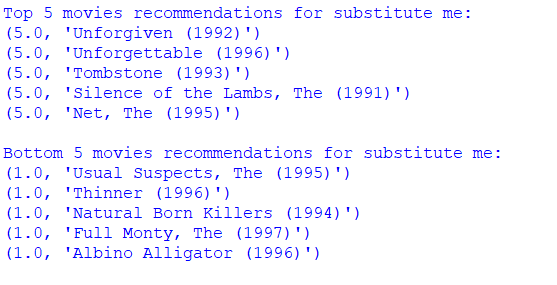
\includegraphics[trim=0 0 0 0, clip, width=\textwidth] {Capture2.PNG}
    \caption{Output for Q3}
    \label{fig2}
\end{figure}

\section*{Discussion}
\emph{Q. Provide a list of the top 5 recommendations for films that the substitute you should see.Provide a list of the bottom 5 recommendations (i.e., films the substitute you is almost certain to hate).}

The question 2's two.py in Listing \ref{2nd:copy} is used to answer this question.

In line 155 to 159, function getRecommendations() was to get my substiture user recommended list, I Used *recommend[0:5] to get first 5 recommendation. This code was gotten from \url{https://github.com/arthur-e/Programming-Collective-Intelligence/blob/master/chapter2/recommendations.py}. 

Top 5 movies recommendations for substitute me, Unforgiven (1992), Unforgettable (1996), Tombstone (1993), Silence of the Lambs, The (1991), Net, The (1995). Bottom 5 movies recommendations for substitute me,in line 159 *recommend[len(recommend)-5:len(recommend)] used it to extract the bottom 5 movie recommendations for substitute me Usual Suspects, The (1995), Thinner (1996), Natural Born Killers (1994), Full Monty, Albino Alligator (1996).

\section*{Q4}
Choose your (the real you, not the substitute you) favorite and least favorite film from the data.

For each film, generate a list of the top 5 most correlated and bottom 5 least correlated films.

Q: Based on your knowledge of the resulting films, do you agree with the results? In other words, do you personally like/dislike the resulting films?

If you have not heard of the recommended movies, search for the movie's trailer on YouTube and watch it before you answer. If you do this, include the link to the trailer in your report. For example, the trailer for "Top Gun (1986)" was found by searching for "top gun 1986 trailer" on Google.
\subsection*{Answer}
\clearpage
\begin{figure}[h]
    \centering
    % trim and clip are used to crop the image, trim=left bottom right top
    % width sets max width, height will be scaled appropriately
    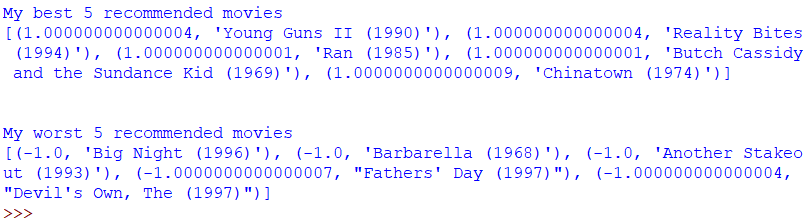
\includegraphics[trim=0 0 0 0, clip, width=\textwidth] {Capture3.PNG}
    \caption{Output for Q4}
    \label{fig2}
\end{figure}

\section*{Discussion}
The question 2's two.py in Listing \ref{2nd:copy} is used to answer this question.

I first transformed the prefs dictionary to movies. I then selected my best (Vampire in Brooklyn (1995)) movie from the whole list in u.data. The function topMatches and bottomMatch handled the result of the questions 3.

\emph{Q: Based on your knowledge of the resulting films, do you agree with the results?  In otherwords, do you personally like/dislike the resulting films?}

Top 5 movies recommend from (Vampire in Brooklyn (1995): \emph{Young Guns II (1990) \url{https://www.youtube.com/watch?v=r-FmfxLy7fo} I like this good old movie.\\ Reality Bites (1994)  \url{https://www.youtube.com/watch?v=xDYGo0UgIVM} It seem interesting and I would watch it. Just an average movie for me.\\ Ran (1985) \url{https://www.youtube.com/watch?v=YwP_kXyd-Rw} I love this one also, war action my favorite.  \\ Butch Cassidy and the Sundance Kid (1969) \url{https://www.youtube.com/watch?v=YdJW2UxvSFQ} I love cow boys like movies\\Chinatown (1974) \url{https://www.youtube.com/watch?v=20FfiP7g4tU} Quite boring but I would enjoy the detective part to movie }

Worst 5 movies recommended from (Vampire in Brooklyn (1995) \\ \\\emph{Big Night (1996) \url{https://www.youtube.com/watch?v=Yd8gK6EgpLM} It is little boring to me because its a chef movie\\ Barbarella (1968) \url{https://www.youtube.com/watch?v=M-fJg08wBKw} Very old movie and I dont find it interesting at all\\Another Stakeout (1993) \url{https://www.youtube.com/watch?v=Gpm4lGyOVYc} I like this one action, detective kind of movies\\Fathers’ Day(1997) \url{https://www.youtube.com/watch?v=xsQfKt08Xlk} Not an interesting movie, too boring.\\ Devil’s Own, The (1997)\url{https://www.youtube.com/watch?v=xZiWSY2SjAM} \ I completely love the action in this movie just the first second of seeing it. As usual war movies gets me all the time.}
\section*{References}
\begin{itemize}
    \item {\url{https://github.com/arthur-e/Programming-Collective-Intelligence/blob/master/chapter2/recommendations.py}}
     \item {\url{https://www.example.com/reallyreallyreally-extra-long-URI/}}
     \item {\url{https://gis.stackexchange.com/questions/180933/how-to-slice-all-elements-in-a-list-to-a-certain-length}}
     \item {\url{https://stackoverflow.com/questions/32448414/what-does-colon-at-assignment-for-list-do-in-python/32448477}}
     \item {\url{http://www.hpc-carpentry.org/hpc-python/04-dicts/index.html}}
     \item {\url{https://www.kite.com/python/answers/how-to-append-an-element-to-a-key-in-a-dictionary-with-python}}
\end{itemize}
\end{document}
\end{document}
\end{document}
